
\section{Experimental results}
\label{sec:exp}

{\em\color{gray} Need to present here both practical results that illustrates the outcome of our solution and how it benefits ... eg show a case where new goals are introduced as we go along}

{\em\color{gray} Also need some analysis -- potentially numerical -- on the overhead and impact fo both solutions relative to each other but also potentially to a more direct classic approach. 
To finally discuss why one solution was preferred on our system} 

Our experiment follows that of the original plan given in
Fig. \ref{fig:ex:plan}. At the beginning, the agent wants to {\em Buy}
an apple and it has to be {\em Home} by the end of the mission. We
implemented this on our executive with plans being produced by the
europa planning engine \cite{frank2003}.\fcomment{I think it is
  important o give at least dome indication of the kind of tools used.
  this should be enough as it is not really giving away that we used
  trex}. Figure \ref{fig:ex:mixed1}
demonstrate the resulting plan from our algorithm and will guide our
explanation. Both algorithms will result in the same execution of the
plan but their approach is quite different.

\begin{figure}
  \centering
  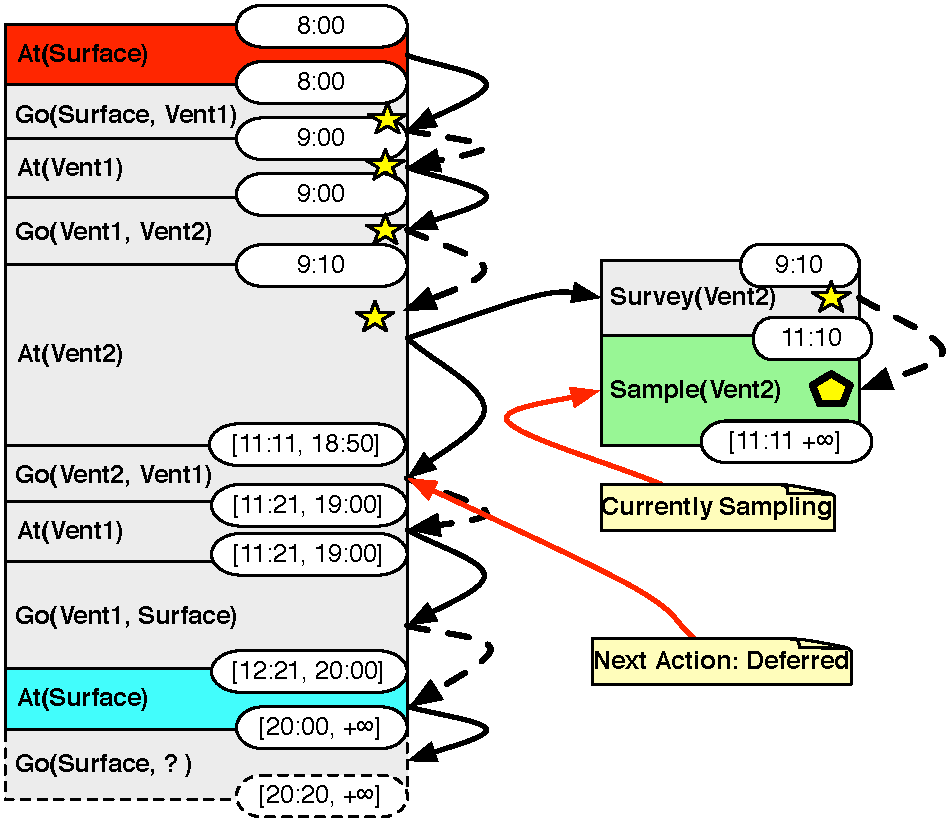
\includegraphics[width=0.8\columnwidth]{figs/example_MixedInitial}
  \caption{Our algorithm solution for the plan from
    Fig. \ref{fig:ex:plan}. Stars indicate tokens that were marked
  as ``proactive''.}
  \label{fig:ex:mixed1}
\end{figure}

For Algorithm \ref{DispatchToken}, the search is quite straight
forward. For example in Fig. \ref{fig:ex:mixed1}, if we are {\em At
Home} then the next {\em Go} token will be dispatched. Because the
search will follow the causal links forward, where upon, it will find
the goal {\em Have Apple} resulting in dispatching proactively.
Similarly, this happens for all of the tokens that are starred. The
rest of the tokens are deferred for later dispatching. The resulting
agent stays at the {\em Grocery} rather than heading {\em Home}
immediately like in Fig. \ref{fig:ex:proactive}.

For the distributed algorithm approach, each token is checked during
the creation of the plan to see if it is an external goal in
$\Phi_{ge}$, or connected to one through a causal link. When the {\em
Have Apple} is checked, we immediately find that it is a goal. We then
follow the reverse causal link and find {\em Buy Apple}.  However to
better illustrate the algorithm, we can imagine that only the {\em Buy
Apple} has been causally connected to the goal so far. Therefore, we
only star those two tokens. The path from {\em Home} to {\em Clothing}
to {\em Grocery} has yet to be built. When the path has finally been
built and {\em At Grocery} is checked our algorithm searches one
causal link and finds {\em Buy Apple} which is starred. The search
then follows the reverse causal link and stars the rest of the
path. The starred tokens will then be proactively dispatched while the
non-starred tokens will be deferred until later. Having similar
results to Algorithm \ref{DispatchToken}.

\begin{figure}
  \centering
  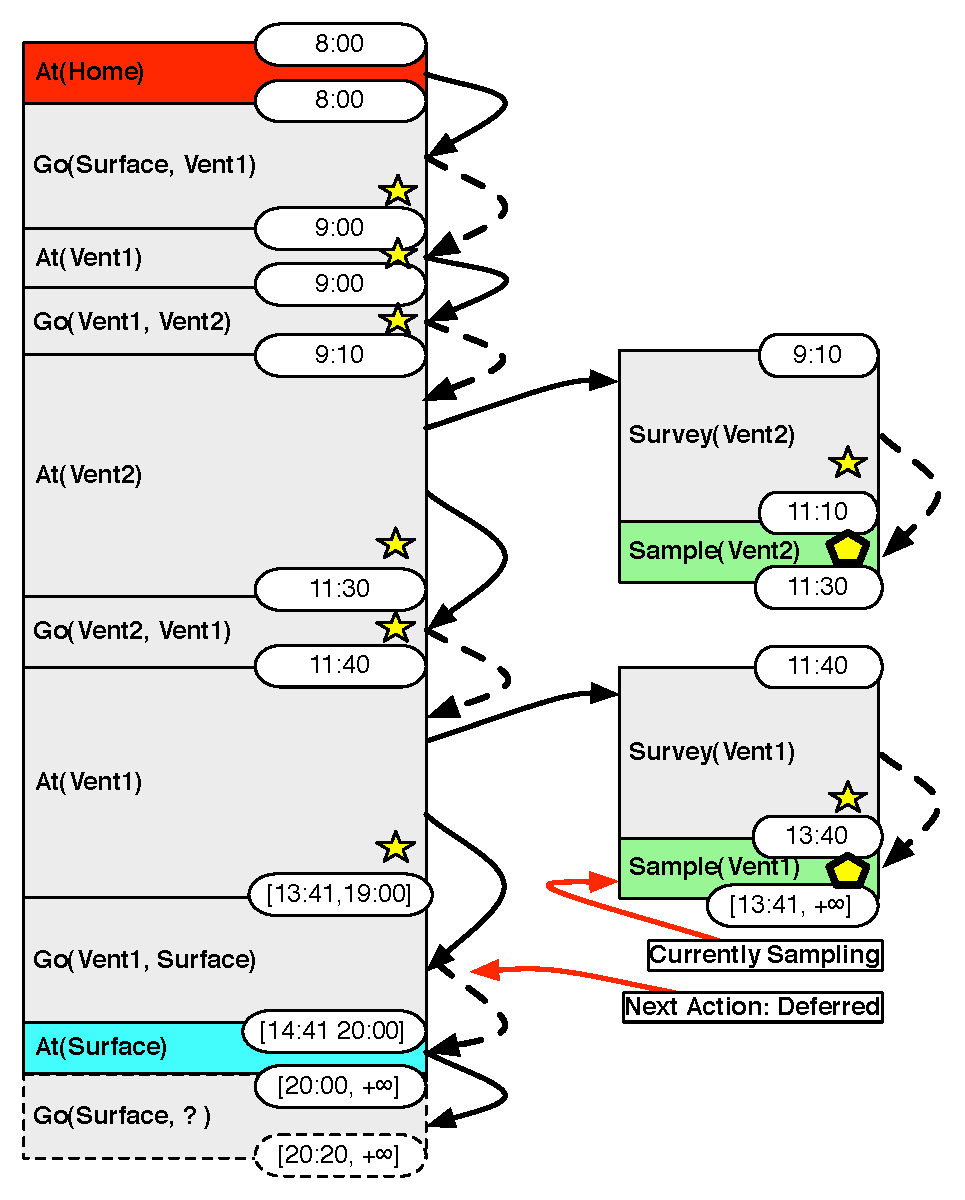
\includegraphics[width=0.8\columnwidth]{figs/example_MixedUpdate}
  \caption{Our algorithm solution after receiving external request for the plan from Fig. \ref{fig:ex:mixed1}}
  \label{fig:ex:mixed2}
\end{figure}

Our reasoning for keeping the agent at the {\em Grocery} is that
nothing is requiring it to go {\em Home} as soon as possible and that
more external requests may come in the near future. To demonstrate
this imagine that while the agent is at the {\em Grocery} it gets a
call at 9:00 asking it to buy a shirt.  We show the resulting plan in
Fig. \ref{fig:ex:mixed2}. Again, both algorithms will result in the
same conclusion. Algorithm \ref{DispatchToken} will search from {\em
Go(Grocery, Clothing)} and will now find {\em Have Shirt}. The
distributed algorithm will find and star the new tokens when the plan
gets updated. The resulting new starred tokens will be proactively
dispatched.

As the end of the day approaches, the agent will need to start heading
home. At 19:40 both algorithms will find that the {\em Go(Clothing,
Home)} is still not connected to a goal but that the upper bound time
for starting the token has been reached. Therefore, we will dispatch
the token because it has become necessary for completing the plan.
After getting {\em Home}, the plan shows that the agent will then {\em
Go(Home, ?)} (dashed in the figures). This is an artefact resulting
from the plan model which specifies that a {\em At} token is followed by a {\em Go}. 
However, our algorithm will not be dispatch this token as 
it is not connected to a goal and its upper bound start time
($+\infty$) will not be met.



%%% Local Variables: 
%%% mode: latex
%%% TeX-master: "aaai13"
%%% End: 
